\documentclass{article}
\usepackage[utf8]{inputenc}
\usepackage{geometry}
\usepackage{graphicx}
\usepackage{float}
\usepackage{listings}
\usepackage{xcolor}
\usepackage{tcolorbox}
\usepackage{hyperref}
\geometry{margin=1in}

\lstset{
    basicstyle=\ttfamily\small,
    breaklines=true,
    frame=single,
    backgroundcolor=\color{gray!10},
    columns=flexible
}

\lstdefinestyle{python}{
    language=Python,
    keywordstyle=\color{blue}\bfseries,
    commentstyle=\color{green!60!black},
    stringstyle=\color{red}
}

\lstdefinestyle{bash}{
    language=bash,
    keywordstyle=\color{blue}\bfseries,
    commentstyle=\color{green!60!black}
}

\lstdefinestyle{yaml}{
    basicstyle=\ttfamily\small,
    keywordstyle=\color{blue}\bfseries,
    commentstyle=\color{green!60!black}
}

\title{Test automation using Selenium, BrowserStack, and GitHub}
\author{Souvik Sarkar \\ \texttt{sounix000@gmail.com}} % Applied your signature author block
\date{October 24, 2022}

\begin{document}

\maketitle

\section*{Context}

\subsection*{Challenges in QA automation}

Automated testing of modern websites and mobile applications poses the following primary challenges:

\begin{itemize}
    \item The tests must run on numerous combinations of devices and browsers in parallel to speed up the process
    \item The tests must be triggered for each new build of the application, or for each new code submission by developers
    \item Logging and observability of test runs must be transparent, and the test results accessible from a single platform
\end{itemize}

\subsection*{Browserstack's offerings}

BrowserStack solves these problems by offering the following:

\begin{itemize}
    \item A large collection of devices and browser versions on which you can run your tests
    \item Support for almost all common programming languages and testing frameworks
    \item Easy integration of large test suites with the BrowserStack platform
    \item Comprehensive and detailed reports and logs for each test session in a single dashboard
    \item Support for automated testing pipelines for all common CI/CD technologies
    \item Intuitive management of users, permissions, and large scale testing infrastructure
    \item Detailed documentation and support for everything you can do with BrowserStack
    \item Transparent and reasonable pricing for individual users, small teams, and enterprises
\end{itemize}

\section*{Objectives}

This tutorial helps you familiarize with BrowserStack's capabilities, so that you can easily adopt BrowserStack for testing websites and mobile applications. In particular, you will learn about the following:

\begin{itemize}
    \item Creating and running a test automation script using Python and Selenium on your local machine. The script automatically tests signing in to Amazon's website.
    \item Adapting the script to use BrowserStack's capabilities, and running tests remotely on BrowserStack
    \item Automating the running of tests using GitHub Actions for each modified version of the script
\end{itemize}

\section*{Audience}

The ideal audience for this tutorial are professionals with interest or experience in automated testing of websites and mobile applications.

\begin{tcolorbox}[colback=yellow!5!white,colframe=orange!75!black,title=Warning]
The code samples used in this tutorial are for demonstration only; DO NOT use them in production scenarios.
\end{tcolorbox}

\section*{Prerequisites}

Before starting with test automation, ensure the following:

\begin{itemize}
    \item Git is installed in your local machine. You can download from it from the git-scm website.
    \item You are familiar with Python and Selenium for automated tests.
    \item You have an active GitHub account. If not, sign up for an account.
    \item You have a basic idea about Continuous Integration (CI) pipelines.
\end{itemize}

\section*{Testing on a local machine}

Before running a script on BrowserStack's grid, create and test the simpler version of the script on your local machine.

\begin{tcolorbox}[colback=blue!5!white,colframe=blue!75!black,title=Note]
All command examples and code snippets included in this tutorial have been tested on a local machine running the \texttt{Fedora 35} operating system. Whenever necessary, modify the commands and code snippets according to your machine's operating system and package manager.
\end{tcolorbox}

\subsection*{Installing dependencies on the local machine}

Before creating a test script, ensure that your local machine has all necessary dependencies.

\textbf{Procedure}

\begin{enumerate}
    \item Write the following script in a file \texttt{set\_up.sh} to create a virtual environment and install dependencies.

\begin{lstlisting}[style=bash]
# This script does the following:
# - sets up a Python virtual environment in the Ubuntu runner for GitHub Actions
# - installs all prerequisites for running the `browserstack_script.py` file in the Ubuntu runner for GitHub Actions 
# the file `browserstack_script.py` on a Ubuntu runner.  
#
# You can also run this script to set up your environment and dependencies.
#
# Check out the list of preinstalled packages for Ubuntu 22.04: https://github.com/actions/virtual-environments/blob/main/images/linux/Ubuntu2204-Readme.md

# Set up and activate a Python virtual environment.
# Assumption: You have already checked out the project repository from GitHub.
cd browserstack-assignment/
python -m venv browserstack
source browserstack/bin/activate

# Install selenium v 4.1.0
python -m pip install selenium==4.1.0

# Install python-dotenv package for handling environment variables from the test script
python -m pip install python-dotenv

# Note: Because the selenium webdrivers invoke headless Chrome and Firefox in the remote BrowserStack Cloud, 
# the Ubuntu runner need not have the specific versions of Chrome and Firefox drivers as mentioned in `browserstack_script.py`.
\end{lstlisting}

    \item Run the \texttt{set\_up.sh} script file.

\begin{lstlisting}[style=bash]
$ bash set_up.sh
\end{lstlisting}

    \item Check the version of Google Chrome on your machine by running \texttt{chrome://version/} on the browser's search bar. Note the version, such as \texttt{Google Chrome: 104.0.5112.79 (Official Build) (64-bit)}.

    \item Check the version of any \texttt{chromedriver} package installed on your system.

\begin{lstlisting}[style=bash]
$ chromedriver --version
ChromeDriver 96.0.4664.45 (76e4c1bb2ab4671b8beba3444e61c0f17584b2fc-refs/branch-heads/4664@{#947})
\end{lstlisting}

    \item If the version of the \texttt{chromedriver} package is older than the Google Chrome version, remove the \texttt{chromedriver} package.

\begin{lstlisting}[style=bash]
$ which chromedriver
~/bin/chromedriver

$ rm ~/bin/chromedriver
\end{lstlisting}

    \item Install the \texttt{chromedriver} package that matches the Google Chrome version.
    \begin{itemize}
        \item Download the correct version for your system from the Chromium website.
        \item Unzip the downloaded file and navigate to the resulting directory.
        \item Copy the \texttt{chromedriver} binary to any location supported by your \texttt{\$PATH} variable.
    \end{itemize}
\end{enumerate}

\subsection*{Locally running a test script}

\begin{enumerate}
    \item Create a \texttt{.env} file and save your Amazon sign in credentials in the file.

\begin{lstlisting}[style=bash]
AMAZON_EMAIL="<email_registered_with_amazon>"
AMAZON_PASSWORD="<password_for_amazon_account>"
\end{lstlisting}

\begin{tcolorbox}[colback=blue!5!white,colframe=blue!75!black,title=Note]
You can safely use the \texttt{.env} file for storing Amazon sign in credentials, while experimenting and developing the scripts. The \texttt{.gitignore} file has an entry for the \texttt{.env} file to prevent any accidental check ins and wider availability of the secrets.
\end{tcolorbox}

    \item Create a file \texttt{local\_script.py}.

\begin{lstlisting}[style=python]
import os, time # The function time.sleep() helps mask the scripted bot behavior.
from selenium.webdriver import Chrome
from selenium.webdriver.common.by import By
from dotenv import load_dotenv

# Helper function to mimic slow typing by a human
def slow_typing(element, text):
    for character in text: 
        element.send_keys(character)
        time.sleep(0.3)

# URL for Amazon website
# Change it depending on your location
AMZ_URL = "https://amazon.in/"

# Load the environment variables from the .env file
load_dotenv()

# Read sign in credentials for Amazon from the .env file
AMAZON_EMAIL = os.environ.get("AMAZON_EMAIL")
AMAZON_PASSWORD = os.environ.get("AMAZON_PASSWORD")

# Open browser and go to sign in page
browser = Chrome()
browser.get(AMZ_URL)
time.sleep(2)
sign_in_button = browser.find_element(By.ID, "nav-link-accountList")
sign_in_button.click()
time.sleep(2)

# Assumption: There are no two-factor authentication enabled
# Enter the sign in credentials
username_textbox = browser.find_element(By.ID, "ap_email")
slow_typing(username_textbox, AMAZON_EMAIL)
time.sleep(2)

continue_button = browser.find_element(By.ID, "continue")
continue_button.submit()
time.sleep(2)

password_textbox = browser.find_element(By.ID, "ap_password")
slow_typing(password_textbox, AMAZON_PASSWORD)
time.sleep(2)

sign_in_button = browser.find_element(By.ID, "auth-signin-button-announce")
sign_in_button.submit()
time.sleep(5)

browser.close()
\end{lstlisting}

    \item Run the file \texttt{local\_script.py}.

\begin{lstlisting}[style=bash]
$ python local_script.py
\end{lstlisting}
\end{enumerate}

\section*{Integrating the script with browserstack}

After successfully testing the script on your local machine, modify and integrate the script with BrowserStack.

\subsection*{Getting browserstack secrets}

\begin{enumerate}
    \item Sign up for a trial account of BrowserStack.
    
    \item Navigate to your BrowserStack dashboard.
    
    \item From the \textbf{ACCESS KEY} dropdown menu, note the values of the \textbf{User Name} and \textbf{Access Key} fields.
    
    \item In the \texttt{.env} file, add the BrowserStack secrets below the Amazon account credentials and save it.

\begin{lstlisting}[style=bash]
BROWSERSTACK_USERNAME="<your_browserstack_username>"
BROWSERSTACK_ACCESS_KEY="<your_browserstack_access_key>"
\end{lstlisting}

    The final content of the \texttt{.env} file is similar to the following:

\begin{lstlisting}[style=bash]
$ cat .env
AMAZON_EMAIL="<email_registered_with_amazon>"
AMAZON_PASSWORD="<password_for_amazon_account>"
BROWSERSTACK_USERNAME="<your_browserstack_username>"
BROWSERSTACK_ACCESS_KEY="<your_browserstack_access_key>"
\end{lstlisting}
\end{enumerate}

\subsection*{Modifying the test script}

Modify the script to use BrowserStack's capabilities of running parallel tests on numerous device and browser combinations.

The entire modified script named \texttt{browserstack\_script.py} is given below:

\begin{lstlisting}[style=python]
# Import necessary packages
import os, time
from dotenv import load_dotenv
from selenium import webdriver
from selenium.webdriver.chrome.options import Options as ChromeOptions
from selenium.webdriver.firefox.options import Options as FirefoxOptions
from selenium.webdriver.common.by import By
from threading import Thread

# Load the environment variables from the .env file
load_dotenv()

# Name of the build that will run remotely on BrowserStack
# Tests will be organized within this build
BUILD_NAME = "browserstack-build-amazon-sign-in"

# The 'capabilities' array defines various browser, device, and OS combinations for the test to run.
capabilities = [
    {
        "browserName": "chrome",
        "browserVersion": "103.0",
        "os": "Windows",
        "osVersion": "11",
        "sessionName": "Parallel Test Chrome Windows",  # test name
        "buildName": BUILD_NAME  
    },
    {
        "browserName": "firefox",
        "browserVersion": "102.0",
        "os": "Windows",
        "osVersion": "10",
        "sessionName": "Parallel Test Firefox Windows",
        "buildName": BUILD_NAME
    },
]

# Change browsers
def get_browser_option(browser):
    switcher = {
        "chrome": ChromeOptions(),
        "firefox": FirefoxOptions(),
    }
    return switcher.get(browser, ChromeOptions())

# The run_session() function handles the sign in to Amazon.
# Depending on your location, modify the default value of 
# the argument AMZ_URL.
# This function also assumes that 2-factor authentication is disabled.
def run_session(cap, AMZ_URL="https://amazon.in/"):
    cap["userName"] = os.environ.get("BROWSERSTACK_USERNAME")
    cap["accessKey"] = os.environ.get("BROWSERSTACK_ACCESS_KEY")
    options = get_browser_option(cap["browserName"].lower())
    options.set_capability("browserName", cap["browserName"].lower())
    options.set_capability("bstack:options", cap)
    driver = webdriver.Remote(
        command_executor="https://hub.browserstack.com/wd/hub", options=options
    )
    # Go to Amazon sign in page
    driver.get(AMZ_URL)
    sign_in_button = driver.find_element(By.ID, "nav-link-accountList")
    sign_in_button.click()
    time.sleep(2)
    # Access the sign in credentials
    AMAZON_EMAIL = os.environ.get("AMAZON_EMAIL")
    AMAZON_PASSWORD = os.environ.get("AMAZON_PASSWORD")
    # Enter email and continue
    username_textbox = driver.find_element(By.ID, "ap_email")
    username_textbox.send_keys(AMAZON_EMAIL)
    time.sleep(2)
    continue_button = driver.find_element(By.ID, "continue")
    continue_button.submit()
    time.sleep(2)
    # Enter password and submit
    password_textbox = driver.find_element(By.ID, "ap_password")
    password_textbox.send_keys(AMAZON_PASSWORD)
    time.sleep(2)
    sign_in_button = driver.find_element(By.ID, "auth-signin-button-announce")
    sign_in_button.submit()
    time.sleep(2)
    print("Sign in test complete.")
    driver.quit()

# The Thread() function takes run_session function and
# each set of capability from the caps array as an
# argument to run each session in parallel.
for cap in capabilities:
    Thread(target=run_session, args=(cap,)).start()
\end{lstlisting}

\subsection*{Running the modified script on browserstack}

Run the \texttt{browserstack\_script.py} file.

\begin{lstlisting}[style=bash]
$ python browserstack_script.py
\end{lstlisting}

\subsection*{Observing test results in browserstack dashboard}

You can monitor tests, inspect logs, and access other details of test sessions using the BrowserStack dashboard.

\begin{enumerate}
    \item In your BrowserStack dashboard, select the build from the \textbf{All Builds} drop down list on the left navigation pane.
    
    \item Check the status of the sessions for the selected build.

    \begin{figure}[H]
        \centering
        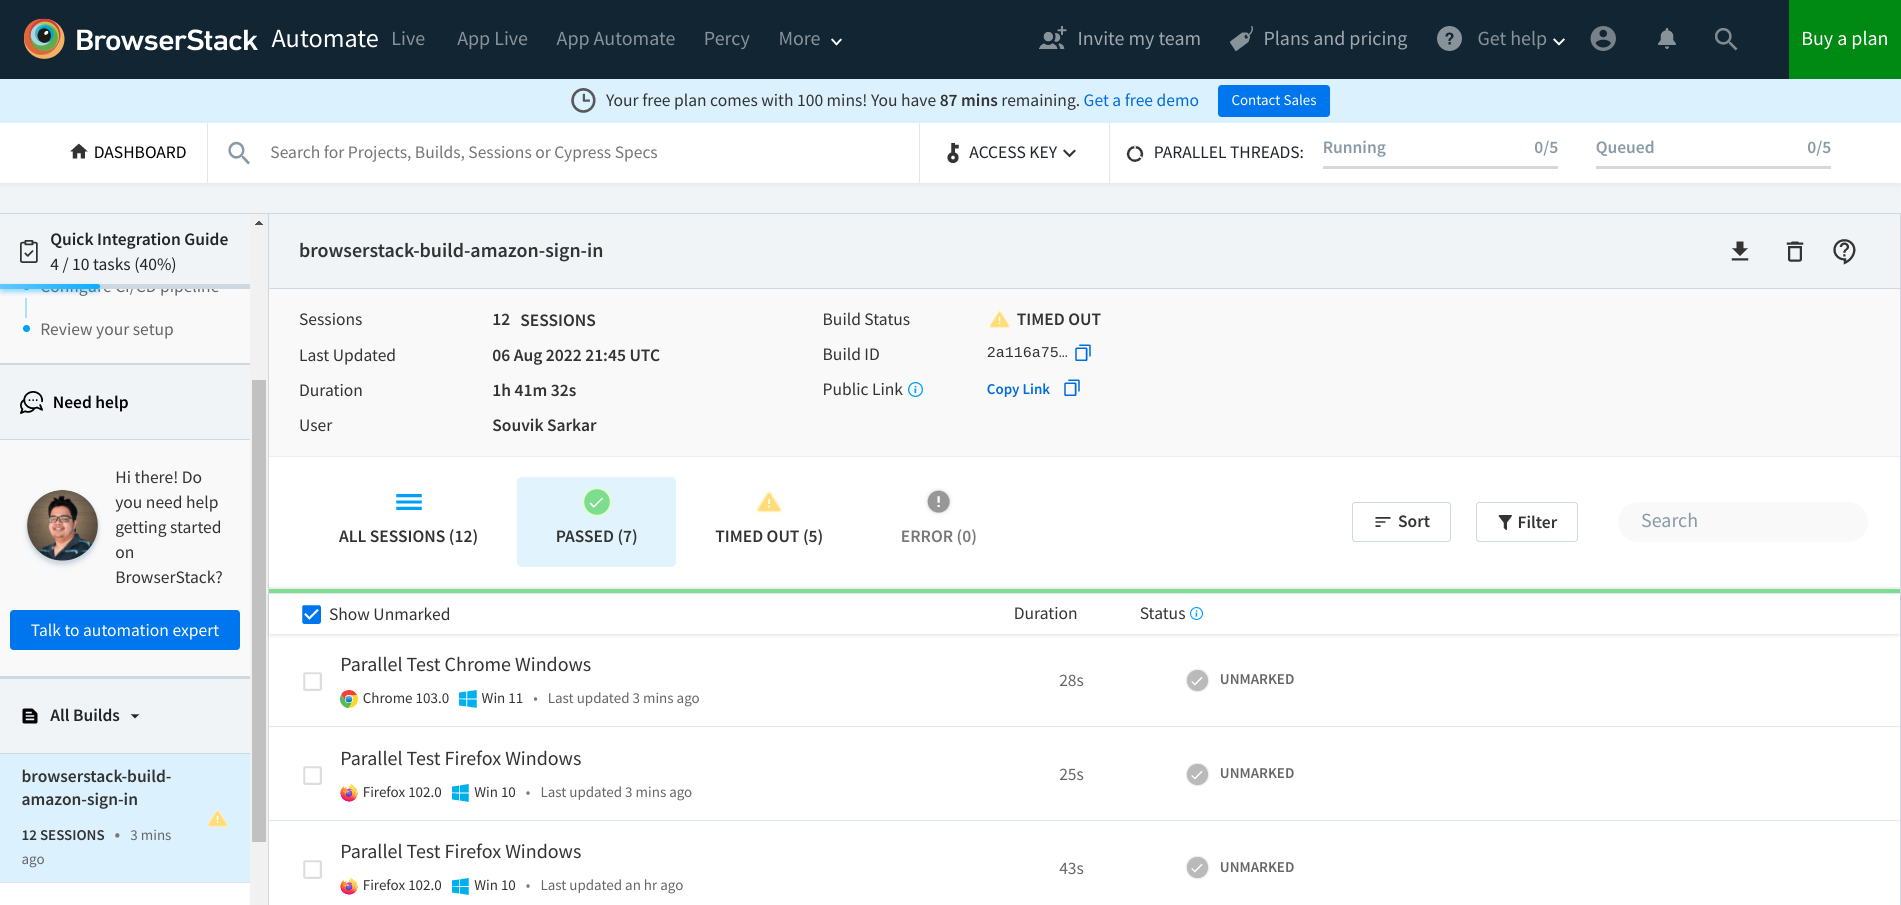
\includegraphics[width=0.8\textwidth]{images/browserstack_builds.png}
        \caption{BrowserStack Dashboard}
        \label{fig:builds}
    \end{figure}
\end{enumerate}

\section*{Automatically running the modified script using github actions}

Using GitHub Actions, set up a CI pipeline such that each push or pull request to the project's GitHub repository triggers the tests to run on BrowserStack.

\begin{enumerate}
    \item Create a \texttt{.gitignore} file with the following content to prevent the environment secrets from getting pushed to a remote repository on GitHub:

\begin{lstlisting}[style=bash]
$ echo ".env" >> .gitignore
\end{lstlisting}

    \item Create a GitHub repository named \texttt{browserstack\_automation} for the project and push the local project to the remote repository.

\begin{lstlisting}[style=bash]
$ git init
$ git add --all
$ git commit -m "first commit"
$ git branch -M main
$ git remote add origin git@github.com:<username>/browserstack_automation.git
$ git push -u origin main
\end{lstlisting}

    \item In your repository on GitHub, navigate to \textbf{Settings} $\rightarrow$ \textbf{Secrets} (left navigation pane) $\rightarrow$ \textbf{Actions} $\rightarrow$ \textbf{New repository secret}.
    
    \item Add your BrowserStack secrets that are available in the \texttt{.env} file of your project directory.
    \begin{itemize}
        \item Enter \textbf{Name}: \texttt{BROWSERSTACK\_USERNAME}, \textbf{Value}: \texttt{<your\_browserstack\_username>}, and click \textbf{Add secret}.
        \item Enter \textbf{Name}: \texttt{BROWSERSTACK\_ACCESS\_KEY}, \textbf{Value}: \texttt{<your\_browserstack\_access\_key>}, and click \textbf{Add secret}.
    \end{itemize}
    
    \item In the repository root, create a \texttt{.github/workflows/browserstack\_actions.yml} file that defines the GitHub Actions workflow.

\begin{lstlisting}[style=yaml]
name: 'BrowserStack GH Actions Test'
on: [push, pull_request]
jobs:
  ubuntu-job:
    name: 'BrowserStack Test on Ubuntu'
    runs-on: ubuntu-latest  # Can be self-hosted runner also
    steps:

      - name: 'BrowserStack Env Setup'  # Invokes the setup-env action
        uses: browserstack/github-actions/setup-env@master
        with:
          username:  ${{ secrets.BROWSERSTACK_USERNAME }}
          access-key: ${{ secrets.BROWSERSTACK_ACCESS_KEY }}

      - name: 'BrowserStack Local Tunnel Setup'  # Invokes the setup-local action
        uses: browserstack/github-actions/setup-local@master
        with:
          local-testing: start
          local-identifier: random

      - name: 'Checkout the repository' # Uses an action from GitHub marketplace to check out the repository
        uses: actions/checkout@v2

      - name: 'Setting up the runner' # Sets up a Python virtual environment and installs prerequisites
        run: bash set_up.sh

      - name: 'Running test on BrowserStack'  # Invokes the actual test script that would run on BrowserStack browsers
        run: python3 browserstack_script.py  

      - name: 'BrowserStackLocal Stop'  # Terminating the BrowserStackLocal tunnel connection
        uses: browserstack/github-actions/setup-local@master
        with:
          local-testing: stop
\end{lstlisting}

    \item To test the GitHub Actions workflow, make a minor modification in the project and push the changes to GitHub.

\begin{lstlisting}[style=bash]
$ git add <modified_file>
$ git commit -m "Testing GitHub Actions"
$ git push
\end{lstlisting}

    \item In your GitHub repository, navigate to \textbf{Actions} $\rightarrow$ \textbf{<your\_GitHub\_Actions\_job>} and observe the job logs.

\begin{tcolorbox}[colback=blue!5!white,colframe=blue!75!black,title=Note]
One of the common reasons of failure for \texttt{browserstack\_actions.yml} workflow is the the following error: \texttt{ModuleNotFoundError: No module named 'dotenv'}.

\begin{figure}[H]
    \centering
    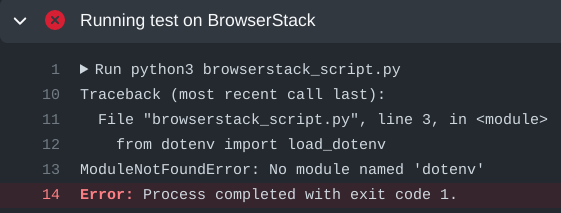
\includegraphics[width=0.8\textwidth]{images/dotenv_error.png}
    \caption{Dotenv error in GitHub Actions}
    \label{fig:dotenv-error}
\end{figure}

The failure happens due to this bug: issue\#273.
The bug is not easily reproducible, and currently has no known solutions that are universally applicable.
\end{tcolorbox}

    \item In your BrowserStack dashboard, select the GitHub Actions build from the \textbf{All Builds} drop down list on the left navigation pane, and observe the test status.
\end{enumerate}

\hrule
\begin{tcolorbox}[colback=gray!5, colframe=blue!50, title=\textbf{Note}]
A modified and hopefully better version of this project is available at \url{https://github.com/sounix000/browserstack-qa-automation}.
\end{tcolorbox}

\end{document}